\section{Implementation on SLang}
\label{sec:implementation_slang}

In the implementation on SonarJava, we had access to the front end of the checker, with a complete tree, a control flow graph and the symbol resolution available.
The first step to implement it on \slang{} is to identify what nodes and structures we need in order to implement everything required for this check.

\subsection{Required Nodes}
\label{subsec:nodes}

The particularity of \slang{} is that it is incomplete. 
The intermediate representation does not need to include all node types in order to work, only the one needed for the checks are mapped. 
We therefore have to make sure that we have all the nodes needed in \slang{} for the implementation of the checker.

\begin{table}[h]
	\caption{Nodes needed for the null pointer dereference check}
	\label{table:nodes-needed}
	\begin{tabular}{|c|c|c|}
		\hline
		\bf Checker specific & \bf Needed for CFG & \bf Others  \\ \hline
	    Binary operation & If/else & Variable declaration \\
		Identifier & Switch & Function invocation \\
		Assignment & Exception handling, throw  & Function declaration \\
		Litteral : Null & Loops & Class declaration \\
		Member select & Jump (break, continue, …) & \\ \hline
	\end{tabular}
\end{table}

Table \ref{table:nodes-needed} shows the nodes needed in order to implement the different parts of the checker.
The first column lists the nodes needed to recognize the different structures used in the checker. 
The interesting node is the \emph{Member Select}, in fact, to identify when a pointer is used, we will only use this node: we do not need to know anything about the context in which the pointer is used, just that it is dereferenced at some point.
When a function is called without a member selection, the tree will be an identifier (name of the function) and a list of argument, but in the case of a pointer use, the tree corresponding to the identifier will be a member selection, that we will use in the checker.
By doing this, we can detect not only functions invocations, but also fields selections or anything considered as a member selection in the original language.

The nodes needed for the control flow graph are the ones expected for identifying the control flow of a program, they are common in all languages and already implemented in \slang{}. 
The way we handle them will be described in subsection \ref{subsec:cfg_on_slang}.
The last column describes other nodes needed indirectly by the checker:
\begin{enumerate}
	\captionsetup[lstlisting]{format=listingEnum, labelfont=white, textfont=white, singlelinecheck=false, margin=0pt, font={bf,footnotesize} }
	\item \textbf{\textit{Variable declaration}} \newline
	\lstinputlisting[label={lst:local-scope-in-while},
	caption=Local scope inside a loop who shadows a field]{code/local-scope-in-while.scala}
	
	In section \ref{subsubsec:identifying_local_variable}, we are going to describe how we perform a naive semantic, assumed inside the check.
	In this semantic, we are not going to be able to differentiate if two pointers having the same name refer to the same declaration.
	The idea to better support this limitation is to kill the pointer in the analysis when we see a declaration, the same way as when we see an assignment.
	In listing \ref{lst:local-scope-in-while} the pointer is used at line $\#1$ and check for \emph{null} at line $\#4$, but the two identifier \emph{p} do not refer to the same symbol.
	In this case, removing \emph{p} from the set when it is declared at line $\#3$ will enable us to remove the false positive.

	\item \textbf{\textit{Function invocation}} \newline
	\lstinputlisting[label={lst:function-invocation-support},
	caption=Pointer used as a parameter of a function call]{code/function-invocation-support.scala}
	
	As discussed before, we do not need explicitly function invocation, only member selection. 
	Due to the way we handle nodes not translated, explained in section \ref{subsec:how_to_deal_with_native}, we will add function invocation support.
	Listing \ref{lst:function-invocation-support} illustrates the situation which we can now report.
	
	\item \textbf{\textit{Function and Class declaration}} \newline
	As our checker is only ran inside functions, we need function declaration to have our starting point. 
	We also use this to improve our semantic, using the fact that the variable used inside a nested function is not checked.
	
	Class declaration is used for the same idea as the function declaration, variables declared in a nested class are assumed to be in another scope.
\end{enumerate}

\subsubsection{Other nodes not supported}
\label{subsubsec:other_nodes_not_supported}

In section \ref{subsec:other_way_to_add_belief}, we saw multiple ways to add the belief that a \emph{null} pointer can be raised. 
\slang{} does not have arrays, we could expect not to find all issues coming from them. 
The length of the array, in \slang{}, is represented as a member select, and can therefore be supported.
Accessing or modifying the fields of \emph{null} as if it were an array is however not supported.
It will lead to false positives, but the situation seems to be uncommon.

\subsection{Control Flow Graph on SLang}
\label{subsec:cfg_on_slang}

\slang{} already has every control flow statement represented in the language, we can already start to build it the same way we would do it for any other language. 
In fact, the current implementation is greatly inspired by the one of SonarPHP \cite{SonarPHP:2019:Online}, also developed at SonarSource.
To build the control flow graph, we are going to use two main kinds of basic blocks:

\begin{enumerate}
	\item \textbf{\textit{CFG Block}} \newline 
	This is the foundation of all basic block of the graph, it contains four fields:
	\begin{enumerate}
		\item \textbf{\textit{Predecessors}} \newline
		List of nodes that may be executed \textbf{before} the current block.
		\item \textbf{\textit{Successors}} \newline
		List of nodes that may be executed \textbf{after} the current block.
		\item \textbf{\textit{Elements}} \newline
		List of instruction executed one after the other in this basic block. 
		\item \textbf{\textit{Syntactic Successor}} \newline
		List of node following the current block if no jump is applied. 
		This is not directly needed for our check, but it may be required in the future.
	\end{enumerate}
	\item \textbf{\textit{CFG Branching Block}} \newline 
	This interface represents blocks including branching instruction, where the flow depends on the result of a Boolean expression. 
	It inherits from CFG Block and has a true and false successor block reference in addition to the simple block.
	\newline 
\end{enumerate}
This is the only two interfaces needed, we can now start to build the graph.

\subsubsection{Building the control flow graph}
\label{subsubsec:building_the_graph}
Since we are going to build a graph for the content of a function, our starting point will be the list of the elements of the function.
We are going to start from the end of the execution, using a bottom-up approach.
It enables us to always know the successor of the node that we are currently building, making easier to build the different instructions containing control flow.
We start by creating an \emph{END} node, containing no element and represents the end of the execution.
We will then recursively build the graph by matching on the type of the tree.

\begin{enumerate}
	\captionsetup[lstlisting]{format=listingEnum, labelfont=white, textfont=white, singlelinecheck=false, margin=0pt, font={bf,footnotesize} }
	\item \textbf{\textit{Block and other nodes}} \newline 
	\label{subsubsec:block_and_others}
	The simplest tree we will face are the blocks, they represent a list of statements.
	We can therefore directly recursively build the graph for all children, recursion that will add the content of the block inside the current basic block. 
	This behavior can also be applied to other known trees which do not change the flow of execution, as a default case.
	The only difference is that we are also going to add the current tree to the elements after having built the graph for the children, in order to keep useful information. 
	For example, having a list of identifiers is not useful if we do not know that they are linked together by a binary expression, we will therefore add both the binary expression and the children to the elements of the current block.
	
	\item \textbf{\textit{If/Then/Else}} \newline 
	\label{subsubsec:if_then_else}
	This is the typical example implementing a branching block. 
	We will first build the sub flow for the false and true branch, if present, and then construct a branching block with these two new blocks as false and true successors, respectively.
	We can now recursively build the condition of the \emph{If} tree from the branching block created before.
	
	\item \textbf{\textit{Loops: For, While, Do-While}} \newline 
	\label{subsubsec:loops_cfg}
	The bottom-up approach makes the creation of the \emph{If} tree straightforward, since we already have built the successor of the tree we are currently building. 
	However, in the case of loops, the flow is not going to continue at the successor, but return at the condition of the loop, a predecessor’s node not built yet.
	To address this situation, we can introduce a \textbf{forwarding block}, a basic block used to store a reference and will not contain any element.
	We can now start to build the loop flow by creating a forwarding block linking to the condition, and build the body with this new block as the successor. 
	Finally, we can build the condition of the loop as a branching block, with the true successor as the body of the loop, and the false as the block following the loop.
	There is one detail we have not addressed yet: break and continue.
	To support these two statements, we are going to use a stack, containing \textbf{breakable} objects. 
	These temporary objects are here to store the link to the condition for emph{continue}, and the end of the loop for \emph{break}.
	Before starting to build the body of the loop, we will push a breakable object to the top of the stack, and pop it once we are done. 
	We use a stack to support nested loop, a break and continue will refer to the first enclosing loop.
	
	The current implementation of \emph{For} loops is the same as \emph{While} loops, as we do not need the exact behavior of a loop for our check, we can accept this approximation.
	For \emph{Do/While} loops, we are going to use the same idea but we are going to start to build the condition before the body.
	
	\item \textbf{\textit{Match Tree}} \newline 
	\label{subsubsec:match_tree_cfg}
	The particularity of a match tree is that it can behave differently depending on the original language.
	For example, in Scala, only one match case can be executed, while in Java, all cases are executed after a matching pattern, until a \emph{break} statement.
	The second example is typically known as fallthrough. 
	In \slang{}, both of them are mapped to the same node, however, identifying which one has the right behavior can be done by storing a flag in the node.
	Non-fallthrough match tree is an easy case, we can build all the cases separately, and create a block having multiples successors.
	
	Fallthrough switch is trickier, we first have to use the same idea as we used for loops: add an object (similar to breakable) to the stack, to store the reference to the block executed after the switch.
	We make the same assumption as we did with loops, that a \emph{break} statements refer only to the closest enclosing match tree. 
	
	The next step is to create a forwarding block for the default case of the match tree, and build the different cases in the reverse order, one after the other. 
	We create one branching block per match cases, with the body of the case as true successor and the next pattern as the false successor. 
	At the same time, we can build the sequence of the body of cases, re-starting each time we see a break.
	
	\lstinputlisting[label={lst:pattern-match},
	caption=Fallthrough pattern matching]{code/pattern-match.scala}
	
	\begin{figure}[h]
		\caption{Listing \ref{lst:pattern-match}'s corresponding CFG }
		\label{figure:pat-mat-cfg}
		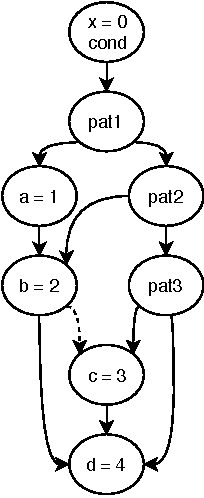
\includegraphics[]{figure/pat-mat-cfg.pdf}
	\end{figure}
	
	Figure \ref{figure:pat-mat-cfg} shows the resulting control flow graph of the code of listing \ref{lst:pattern-match}. We can see that the fallthrough behavior is represented as expected, for example \emph{a = 1} is executed both when \emph{pat1} and \emph{pat2} is \emph{True}.
	
	\item \textbf{\textit{Jump Tree: break and continue}} \newline 
	\label{subsubsec:jump_tree_cfg}
	
	Jump trees are not supposed to appear when we do not expect them.
	If we have an unexpected jump tree, we cannot do anything, and we will directly add it to the current block.
	We will discuss in section \ref{subsec:how_to_deal_with_native} a better solution to support this situation.
	In the usual case, they will appear where we expect them and create an edge from the current block to the head of the stack filled as described in \ref{subsubsec:loops_cfg} and \ref{subsubsec:match_tree_cfg} sections.
	
	\item \textbf{\textit{Return}} \newline 
	\label{subsubsec:return_cfg}
	Again, starting from the end greatly simplifies the support of return statements: we can store a reference to the \emph{END} block created at the beginning, and use it as successor to the block  containing the return expression.
	
	\item \textbf{\textit{Exception Handling Tree and Throw Tree}} \newline 
	\label{subsubsec:exception_handling_cfg}
	In our control flow graph, we are only going to consider exceptions explicitly thrown with a throw statement, and not add an edge to every statement where an exception can occur in reality. \newline
	We are going to start at the end of the exception handling tree. 
	When an exception handling tree is executed, it can result in two possible cases: the exception is caught and the flow can continue, or it is not and the flow goes to the end of the function. 
	To support this behavior, we are going to create a block with two successors: the \emph{END} node and the successor previously created. \newline
	We can then create the \emph{finally} block, if present, and the different catch cases separately, and continue to build the body of the \emph{try} block. 
	At this point we must know where to jump in the case where an exception is thrown. 
	To do this, we will use the same idea as we did with the jump trees: use a stack to push the target of the throw before building the body, and popping it after. 
	If there is no catch block, the target will be the \emph{finally} block, if there is one or more catch block, we will use the first catch case as target. 
	This is an approximation due to the fact that we have no symbol resolution, we cannot know which and where the exception is caught.
	From now, we can know where to jump in the case of a throw three.\newline
	The last detail to take care of is the case where we have a return inside an exception handling tree.
	In this case, the \emph{finally} block is executed after the return. 
	To support this, we will store the exit target on a stack, pushing the reference to the finally block on top of the \emph{END} block previously added.
	
	\item \textbf{\textit{Natives Nodes}} \newline 
	\label{subsubsec:native_nodes_cfg}
	The new challenge comes from the node who is new in \slang{}: the \emph{native node}. 
	The way we deal with native nodes will be described in subsection \ref{subsec:how_to_deal_with_native}.
\end{enumerate}

\subsubsection{Normalization}
\label{subsubsec:normalization_cfg}
The core of the graph is done, but we still need to perform a few modifications in order to have a proper control flow graph. 
First, we are going to remove empty blocks. 
They can be introduced in multiple situations, when we create a temporary forwarding block or when the header of a \emph{For} loop is empty for example.
During the creation of the graph, we only knew the successors of the nodes, we still have to compute the predecessor set. 
Since we have all successors, the task is straightforward. 
Finally, we can create a \emph{START} node, implementing the same behavior as the \emph{END} node, to indicate the beginning of the flow.

\subsection{Data flow analysis}
\label{subsec:data_flow_analysis}

We now have all nodes needed and a control flow graph, we can start the implementation of the checker, which is in fact really similar to the one described in \ref{sec:implementation_java}. 
The main difference is the way we deal with nodes having an unreliable execution order and the identification of local variables.
The former will be described in \ref{subsec:how_to_deal_with_native} and the latter in the next section.

\subsubsection{Identifying local variable}
\label{subsubsec:identifying_local_variable}

In SonarJava, we have access to symbols of identifiers, data that we do not have in \slang{}. 
The current computation of local variables is quite simple: all variable declaration inside the function and all arguments are considered as local variables.
This is a naive version will not work for all language but it is used to show that with a proper semantic computation (name definitions and scoping rules) we could expect results as good as the current naive version. \newline
When we have this set of local variables, we can now check if the variable is in this set before reporting the issues. 
In practice, we could still report the issues not coming from local variables, but this would add some false positives.

\lstinputlisting[label={lst:field-change-value},
caption=Field can change value during a function call]{code/field-change-value.scala}

Listing \ref{lst:field-change-value} shows an example of a false positive due to a function with side-effect changing the value of a field. 
Adding the issues coming from non-local variable double the number of issues found, but most of them are false positives.
Since a variable can be reassigned between the use and the check of a pointer, these new issues do not exactly respect the original description, we are not going to report them.

\subsection{How to deal with native nodes in a CFG based checker?}
\label{subsec:how_to_deal_with_native}

It is finally time to explain how we are going to deal with the native nodes.
For our concern, we will see the native nodes as a node that we do not know anything about, with a list of children.

\lstinputlisting[label={lst:ternary-expression-belief},
caption=Simple ternary expression]{code/ternary-expression-belief.scala}

\begin{figure}[h]
	\caption{\slang{} AST from the code of listing \ref{lst:ternary-expression-belief}}
	\label{figure:ternary-ast}
			\Tree[.... 
				[.\color{red}Native
				[
					\textit{true}
					\textit{b}
					\textit{p.toString()}
				]
				]
				\textit{p == null}
				]
\end{figure}
Figure \ref{figure:ternary-ast} shows the result of the \slang{} tree created from the code from listing \ref{lst:ternary-expression-belief}. 
In this example, we assume that we do not have ternary expression in \slang{}, and that they are not mapped to \emph{If/Then/Else} statement. 
We will use ternary expression of Java to represent the problem, but the construction can be any native nodes coming from any original language. \newline
The problem is that we must represent the control flow of an unknown node.
We cannot trust the evaluation order of the children of the native nodes, as it can be arbitrary. 
The first question arising is why do we have to keep the content of a node we do not know anything about? In fact, this is the root of the idea of the native nodes, we are not interested in the node itself, but only in the content.

\begin{figure}[h]
	\caption{CFG with an assignment in a native node}
	\label{figure:cfg-with-assignment-native}
	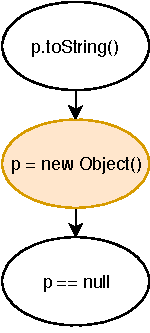
\includegraphics[]{figure/cfg-with-assignment-native.pdf}
\end{figure}

Figure \ref{figure:cfg-with-assignment-native} shows a typical example: in this case, we do not care what exactly happens in this native node (orange node), we just need to know that, at one point, \emph{p} is assigned, even if it is possible that the assignment is never executed.
If it is the case, this will add false negatives, but intuitively, dead code is not common, and will not happen very often.

At this point, we need to keep the content of the native nodes. 
The next step is to define what to do with them. 
A naive solution would be to add the content of the graph in the elements of the basic block, assuming that the evaluation order is not important. 
This is in fact correct for a native node with only one child, where the evaluation order can obviously not change. 
If there are multiple children, we have to add the assumption that all the statements who change the flow of a program are represented in \slang{}. 
This is a reasonable assumption since programming language hardly ever provide an exceptional statement who breaks the control flow, and if it does, we can add it to \slang{} grammar.

\lstinputlisting[label={lst:ternary-expression-example},
caption=Pseudo code with a ternary expression]{code/ternary-expression-example.scala}

\begin{figure}[h]
	\caption{Basic block content of the code in listing \ref{lst:ternary-expression-example}}
	\label{figure:basic-block-content}
	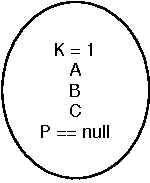
\includegraphics[]{figure/basic-block-content.pdf}
\end{figure}


Listing \ref{lst:ternary-expression-example} some Java pseudo code with the corresponding control flow graph with the naive implementation in figure \ref{figure:basic-block-content}.
Since the ternary expression will be mapped to a native node in \slang{}, if we take the children of the native node in order, we will obtain the execution order of the nodes in figure \ref{figure:basic-block-content}.
It is obviously not correct, as the pointer will be seen as used then checked in this order, but it is not in the real execution.

\begin{figure}[h]
	\caption{CFG with elements coming from natives nodes}
	\label{figure:two-unreliable-cfg}
	\setlength{\tabcolsep}{24pt}
	\begin{tabular}{cc}
		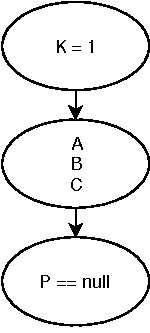
\includegraphics[]{figure/unreliable-cfg-1.pdf}  &
		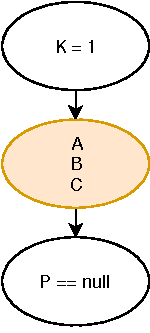
\includegraphics[]{figure/unreliable-cfg-2.pdf}   \\ 
		Split CFG & Split block with unreliable node
	\end{tabular}
\end{figure}

We can therefore not ignore these nodes, and not naively add them to the blocks.
The idea to solve the problem shown before is to put all elements coming from a native node in a separate basic block (figure \ref{figure:two-unreliable-cfg}, left), and mark the block as \textbf{unreliable} (figure \ref{figure:two-unreliable-cfg}, right), shown in orange.
All control flow statement nested inside the native nodes will also lead to an unreliable basic block.\newline
Additionally, we will also mark the whole graph as unreliable. 

This information can now be used by any checker using a control flow graph, not only for the \emph{null} pointer dereference checker.

\subparagraph{How to use this information?}
\label{subsubsec:use_unreliable_information}

This information can be used in different ways to help to define the multiple level of granularity of the implementation of a new checker:

\begin{enumerate}
\captionsetup[lstlisting]{format=listingEnum, labelfont=white, textfont=white, singlelinecheck=false, margin=0pt, font={bf,footnotesize} }
\item \textbf{\textit{Ignore this information}} \newline
In some case, it may make sense to ignore this information, and to treat unreliable nodes as others. 
In our case, we have shown previously that this solution is not suitable, as it produces too many false positives. \newline

\item \textbf{\textit{Don’t run the checker on unreliable CFG}} \newline
This is the opposite of the previous point: in the case where the checker needs to really trust the control flow graph, it can make sense to stop the checker if the graph cannot be trusted.

\begin{table}[h]
	\centering
	\caption{Percentage of native and completely native nodes in the different languages}
	\label{table:slang-native-percentage}
	\begin{tabular}{|c|c|c|c|}
		\hline
		\bf Language & \bf \% & \bf \% of completely native & \bf $\bf N^{\circ}$  of files \\ \hline
		Scala &  41 &  6.25 & 6126 \\ 
		Kotlin &  47 &  6.5 & 26758 \\ 
		Ruby &  39 &  5.2 &  7811 \\ \hline
	\end{tabular}
\end{table}

Table \ref{table:slang-native-percentage} shows the percentage of native nodes in \slang{} after translating open-source projects \cite{SlangSources:2019:Online} to \slang{}. 
The percentage of completely native nodes refers to the nodes having all their children as native. 
If more than $40\%$ of nodes are not translated, this does not mean that our language lacks nodes, but that we do not map some kind of nodes on purpose.
This table shows us that native nodes are not rare, using the above approach will greatly reduce our chance to find any relevant issue as we will, in most of the case, be in the presence of native nodes in the body of a function.

The two approaches described before seems not well-suited for our checker, we may want something between the two extremes.

\item \textbf{\textit{Fine grain}} \newline
We can use the fact that we know if an element comes from a native node or not to define a finer grain implementation of our checker. 
It consists mainly in one modification of the data flow analysis described in section \ref{subsubsec:data_flow_analysis}: we do not add a pointer used in an unreliable block to the believed to be \emph{non-null} set, the equation \eqref{eqn:dataflow3} therefore becomes:

\begin{equation}\label{eqn:new_dataflow4}
newGen(n) = \parbox{7cm}{pointer used in the node n\newline exept if marked as unreliable}
\end{equation}

\lstinputlisting[label={lst:fine-grain-1},
caption=First example of finer grain behavior]{code/fine-grain-1.scala}

\lstinputlisting[label={lst:fine-grain-2},
caption=Second example of finer grain behavior]{code/fine-grain-2.scala}

With this idea, we are now avoiding to report any issue for the two correct pseudo code from listing \ref{lst:fine-grain-1} and \ref{lst:fine-grain-2}. Since ternary expressions are unreliable, we will not consider \emph{p} as used, even though it may look like in the control flow graph.

\lstinputlisting[label={lst:fine-grain-3},
caption=Third example of finer grain behavior]{code/fine-grain-3.scala}

In listing \ref{lst:fine-grain-3}, the real evaluation order use \emph{p} and then check it for \emph{null}. 
This code is not reported by our tool despite the fact that it should be. This is a false negative.\newline

\lstinputlisting[label={lst:fine-grain-4},
caption=Fourth example of finer grain behavior]{code/fine-grain-4.scala}

In addition, the implementation will still report issues inside native nodes.
For example, in listing \ref{lst:fine-grain-4}, we can see that the pointer \emph{p} is used, and then checked for \emph{null} later in a un-trusted node. 
We do not know what happens in this node, but we can expect that a check for \emph{null} still means that p can be \emph{null}. 
In this example, we report an issue, who is a true positive.
\end{enumerate}

\subsection{Problematic situations}
\label{subsec:other_problematic_situation}
	
We have already presented the main problematic situations, coming from native nodes, but there are still a few cases raising false positives that we have to take care of.

\begin{enumerate}
	\captionsetup[lstlisting]{format=listingEnum, labelfont=white, textfont=white, singlelinecheck=false, margin=0pt, font={bf,footnotesize} }
	\item \textbf{\textit{Boolean short-circuit}} \newline 
	\label{subsubsec:boolean_short_circuit}
	Our current implementation of the control flow graph does not encode the possible path due to Boolean short-circuit. 
	This will lead to a wrong evaluation order, even if the nodes are known. 
	Since the evaluation order is not correct, it makes sense to treat them the same way we do with native nodes.
	We will hence keep all the content of these nodes, to be able to use them in the checkers, but mark them as unreliable. 

\lstinputlisting[label={lst:boolean-short-circuit},
	caption=Problematic situations due to Boolean short circuit]{code/boolean-short-circuit.scala}
	
	With this addition, we are now able to avoid the false negative reported in the two examples of listing \ref{lst:boolean-short-circuit}.
	\pagebreak
	\item \textbf{\textit{Order of evaluation of known nodes}} \newline 
	\label{subsubsec:evaluation_known_nodes}
	In section \ref{subsec:how_to_deal_with_native}, we saw that the order of evaluation of the nodes are critical for our checker.
	When coming from different languages, even known nodes can have different evaluation order, as we have seen an example in section \ref{subsubsec:match_tree_cfg}. 
	The same situation can arise for any statement.
	Hopefully, the solution is often to add the support for the new behavior in \slang{}.
	This trick should be used with caution, the initial goal is to be language agnostic, we should ideally not have to modify \slang{} for every new language we add. 
	The good news is that there is only a limited number of variations possible, since the number of known nodes is fixed (and only a fraction of it in practice). 
	This kind of problems are difficulties hard to anticipate and will arise during the implementation of a new checker, but it is not in itself a strong limitation.
	
	\item \textbf{\textit{Lost Jump Statements}} \newline 
	\label{subsubsec:lost_jump_statement}
	We have seen in section \ref{subsubsec:jump_tree_cfg} that we directly add jump statements to a basic block in the case where we do not expect it, without doing anything special.
	In fact, we face similar uncertainties happening with native nodes, we do not know exactly what is happening, but we can expect that something will go wrong.
	The same arises with jump tree with labels, the way different language deals with label can be arbitrary.
	We cannot assume anything related to them.
	We just know that the statement will change the execution flow in an unreliable way, we will therefore mark the flow generated by this statement as \emph{unreliable}.
\end{enumerate}
